\section{Environment Attribute} \label{sec:env_attr}

As shown in Fig. \ref{fig:env_attribute}, the landscape of agent evaluation environments is characterized by a multidimensional taxonomy of attributes. These underlying attributes change how agents perceive, interact, and make decisions with the environments. To capture the fundamental differences among these environments, it is necessary to analyze them based on their basic mechanics and mathematical formulations. Therefore, we break down the basic attributes of these environments into several key pairs, including \textbf{Symbolic vs. Neural} (\cref{attribute:Symbolic vs. Neural}), \textbf{Open-Loop vs. Closed-Loop} (\cref{attribute:Open-Loop vs. Closed-Loop}), \textbf{Online vs. Offline} (\cref{attribute:Online vs. Offline}), \textbf{MDP vs. POMDP} (\cref{attribute:MDP vs. POMDP}), \textbf{Deterministic vs. Nondeterministic} (\cref{attribute:Deterministic vs. Nondeterministic}), \textbf{Discrete vs. Continuous} (\cref{attribute:Discrete vs. Continuous}), \textbf{Unimodal vs. Multimodal} (\cref{attribute:Unimodal vs. Multimodal}), and \textbf{Single-Agent vs. Multi-Agent} (\cref{attribute:Single-Agent vs. Multi-Agent}). This taxonomy establishes a systematic framework for analyzing these environments, highlighting the diverse complexities and fundamental attributes that shape agent-environment interactions.

\begin{figure*}[t]
    \centering
    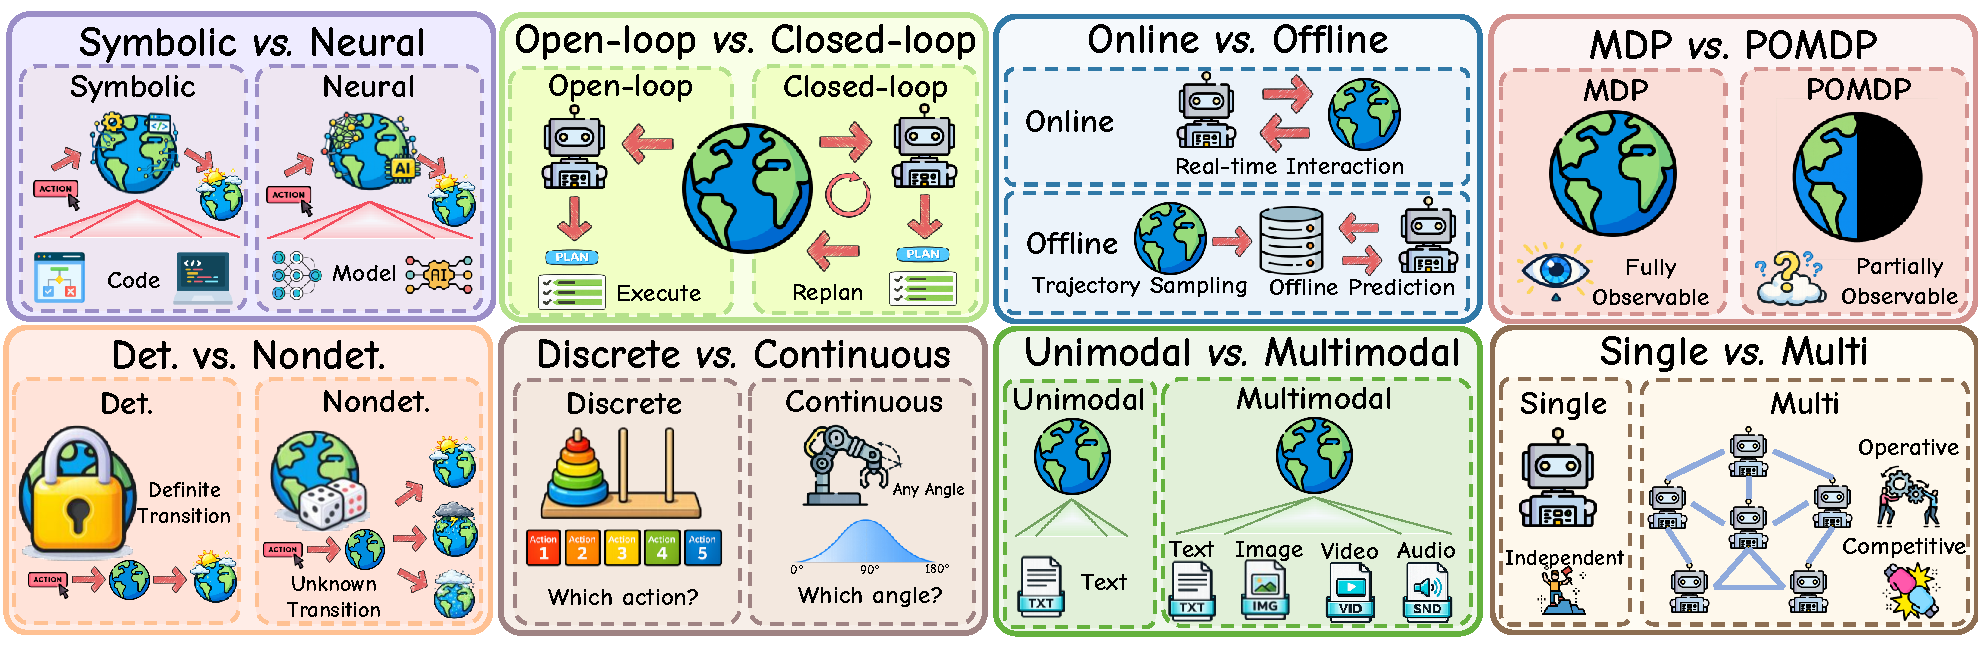
\includegraphics[width=\textwidth]{images/env_attribute.pdf}
    \caption{An overview of environment attributes.} 
    \label{fig:env_attribute}
\end{figure*}

\subsection{Symbolic vs. Neural}
\label{attribute:Symbolic vs. Neural}
The core distinction between these paradigms lies in the underlying implementation of the transition function $\mathcal{P}$ and how the environment dynamics are generated. This determines whether the system relies on programmed code to update the states or uses a neural model to predict future states.

\subsubsection{Symbolic Environment}
In a symbolic environment, the transition dynamics are governed by explicit programmed logic and predefined rules. The transition function $\mathcal{P}(s_{t+1} | s_t, a_t)$ is realized through executing source code, software scripts, or physics engines. As a foundational standard in this paradigm, the planning domain definition language (PDDL) governs transition dynamics through explicit symbolic action schemas, utilizing logical preconditions and deterministic effects to update environment states. While PDDL provides a strict logical foundation, modern environments predominantly realize these transitions through flexible programming code. Agent World Model~\cite{Agent_world_model} synthesizes large executable environments using code-driven backends and SQL databases to ensure reliable state transitions and consistency for agent training. EnvScaler~\cite{EnvScaler} programmatically synthesizes executable tool-interactive environments where transition dynamics and state updates are governed by explicit Python code and predefined rule-based logic. AutoEnv~\cite{AutoEnv} utilizes domain-specific languages and code abstractions to automate the synthesis of executable environments with explicit, programmed transition and reward logic.

\subsubsection{Neural Environment}
In a neural environment, the transition dynamics are approximated by a model parameterized by $\theta$. The transition function $\mathcal{P}_{\theta}(s_{t+1} | s_t, a_t)$ is realized through the forward propagation of these learned parameters, typically utilizing neural networks. This approach often serves as a surrogate simulator to generate state transitions where the true underlying physical rules are unknown or overly complex. WebDreamer~\cite{WebDreamer} uses LLMs as learned world models to simulate web state transitions, approximating environment dynamics through neural network parameters rather than explicit code. DreamGen~\cite{DreamGen} utilizes neural video world models to approximate environment transitions and generate synthetic trajectories for robot training through the forward propagation of learned parameters. WebEvolver~\cite{WebEvolver} employs concurrently optimized LLMs to function as virtual web servers, forecasting future webpage representations based on present conditions and executed actions to synthesize multi-step interaction trajectories.


\subsection{Open-Loop vs. Closed-Loop}
\label{attribute:Open-Loop vs. Closed-Loop}
The core distinction between the two paradigms lies in how the agent utilizes the observation sequence to formulate its actions over time. This determines whether the agent simply executes a fixed plan based on the starting conditions, or continuously adjusts its next steps based on new feedback from the environment.

\subsubsection{Open-Loop Environment}
In an open-loop system, the agent receives only a single initial observation $o_0$ and executes a predetermined sequence of actions. It does not incorporate subsequent feedback from the environment. The policy simplifies to depend on a sequence predetermined from the initial observation $\pi(a_t | o_0)$ in a non-adaptive manner. TaskLAMA~\cite{TaskLAMA} decomposes complex tasks into structured task graphs from initial goal prompts without incorporating real-time environmental observations or adaptive feedback mechanisms. HuggingGPT~\cite{HuggingGPT} adopts a global planning strategy to predetermine a complete task sequence from the initial request without incorporating subsequent feedback from the environment during execution. TaskBench~\cite{TaskBench} assesses task automation capabilities by requiring models to generate a tool invocation graph directly from the initial user instruction, omitting interactive feedback from actual tool execution.

\subsubsection{Closed-Loop Environment}
In a closed-loop system, the agent receives new observations $o_t$ at each time step and adapts its actions accordingly. The policy utilizes the dynamically updating history $h_t$ to make reactive decisions, allowing the agent to respond to environmental stochasticity and correct deviations. Mobile-Bench~\cite{Mobile-Bench} implements an iterative execution framework where agents dynamically update their thoughts and actions based on real-time UI feedback and historical environment observations. MCPVerse~\cite{MCPVerse} utilizes an automated agentic loop where models interact with executable tools and leverage real-time feedback to iteratively refine their planning and multi-step actions. WebWalker~\cite{WebWalker} employs an explore-and-critic framework that iteratively adapts its navigation based on real-time observations and dynamic memory to resolve complex web traversal tasks.

\subsection{Online vs. Offline}
\label{attribute:Online vs. Offline}
The core distinction between the two paradigms lies entirely in the interaction mechanism. This mechanism dictates whether an agent actively drives state transitions through sequential exploration with the environment, or is evaluated solely on its ability to mimic expert behavior from pre-recorded trajectories.

\subsubsection{Online Environment}
In an online environment, the agent actively interacts with the true dynamical system $\mathcal{E}$. At each time step $t$, the agent executes an action $a_t$, and the environment sequentially yields the subsequent observation $o_{t+1}$. The agent evaluates and refines its behavior through real-time feedback. For example, WebArena~\cite{WebArena} provides a suite of fully functional websites where agents interact dynamically and receive real-time feedback to achieve complex tasks. EmbodiedBench~\cite{EmbodiedBench} assesses vision-driven agents through real-time interaction across diverse simulated environments , where models must actively process sequential feedback and visual observations to refine their task execution. Terminal-Bench~\cite{Terminal-Bench} benchmarks agents on interactive, long-horizon tasks within real terminal environments, requiring models to autonomously manipulate containerized systems and refine actions based on sequential execution feedback.

\subsubsection{Offline Environment}
In an offline environment, direct interaction with the system $\mathcal{E}$ is strictly prohibited. The agent relies instead on a static dataset of previously sampled trajectories $\mathcal{D}$. Evaluation is conducted statically by comparing the predicted single step action $\pi(a_t | h_t)$ against the expert action $a^*_t$ from human or strong models, severing the standard sequential feedback loop. For example, Mind2Web~\cite{Mind2Web} evaluates agents on cached snapshots of real-world websites by comparing predicted actions against human-annotated trajectories without real-time sequential feedback. ALFRED~\cite{ALFRED} uses a static dataset of expert demonstrations to evaluate models, comparing predicted actions against human-annotated ground truth without real-time environmental feedback. AndroidControl~\cite{AndroidControl} evaluates agents on a static dataset across apps, measuring single-step action accuracy against expert ground truth rather than through real-time environmental interaction.

\subsection{MDP vs. POMDP}
\label{attribute:MDP vs. POMDP}

The core distinction between these two paradigms lies in the mapping relationship between the environment's state space $\mathcal{S}$ and the agent's observation space $\Omega$. Essentially, this determines whether the agent has full access to everything happening in the environment, or if it must rely on incomplete observations to understand the true situation.

\subsubsection{Fully Observable Environment}
In a fully observable environment, typically formalized as a Markov Decision Process (MDP), the agent has complete and transparent access to the true dynamics. The observation space perfectly aligns with the state space, formally $\Omega = \mathcal{S}$. Here, the observation $o_t$ is entirely identical to the latent state $s_t$, allowing the agent to base its policy strictly on the current state without needing historical context, formulated as $\pi(a_t | s_t)$. For example, KOR-Bench~\cite{KOR-Bench} evaluates reasoning capabilities through tasks where all logical rules and complete problem states are explicitly provided in the text prompt. GVGAI-LLM~\cite{GVGAI-LLM} directly presents the evolving game status and foundational principles through formatted text descriptions during every single step. V-GameGym~\cite{V-GameGym} evaluates LLMs on synthesizing complete visual games from explicit text instructions where the sandbox execution provides transparent access to all underlying game states.

\subsubsection{Partially Observable Environment}
In a partially observable environment, modeled as a POMDP, the agent lacks direct access to the complete latent state. The observation $o_t \in \Omega$ serves as an incomplete or noisy projection of $s_t$, strictly governed by the observation function $\mathcal{O}(o_t | s_t, a_t)$. Consequently, the agent is required to aggregate information across its entire interactive trajectory $h_t$ to infer the underlying state distribution and execute optimal decisions. For example, WebArena~\cite{WebArena} evaluates web agents that observe only the focused tab or a limited viewport. Consequently, agents must rely on their interaction history to infer the full underlying website state. GAIA~\cite{GAIA} evaluates general AI assistants on complex real-world questions where agents must iteratively gather information from a diverse environment. EmbodiedBench~\cite{EmbodiedBench} evaluates multimodal agents in 3D simulated tasks where the complete environment state is hidden , requiring models to make decisions relying entirely on egocentric visual observations and interaction history.


\subsection{Deterministic vs. Nondeterministic}
\label{attribute:Deterministic vs. Nondeterministic}
The distinction between deterministic and nondeterministic environments is characterized by the properties of the transition function $\mathcal{P}$ and the reward function $\mathcal{R}$. Essentially, this determines whether taking a specific action in a given situation always produces the exact same, predictable states, or if the outcome involves randomness and uncertainty.

\subsubsection{Deterministic Environment}
In a deterministic environment, executing a specific action $a_t \in \mathcal{A}$ in a given state $s_t \in \mathcal{S}$ invariably results in a single, predictable next state $s_{t+1}$ and reward $r_t$. Formally, the transition kernel collapses into a deterministic mapping, such that $\mathcal{P}(s_{t+1} | s_t, a_t) = 1$ for exactly one target state. GameTraversalBenchmark~\cite{GameTraversalBenchmark} evaluates planning on static 2D maps where discrete directional actions predictably determine the next state. Baba Is AI~\cite{BabaIsAI} introduces a gridworld puzzle game where manipulating objects and textual rules results in predictable and exact state transitions. 
VSP~\cite{Vsp} features classical maze navigation and block-moving scenarios, which serve as deterministic environments because they are governed by strict, predefined rules where every allowed action yields a guaranteed, predictable outcome.


\subsubsection{Nondeterministic Environment}
In a nondeterministic environment, the environmental dynamics are governed by probability distributions. Taking an action $a_t$ in state $s_t$ results in a next state $s_{t+1}$ that is sampled from the distribution defined by the transition kernel $\mathcal{P}(\cdot | s_t, a_t) \in \Delta(\mathcal{S})$. Consequently, the identical state-action pair $(s_t, a_t)$ can yield different resulting states and rewards across independent interactions. Furthermore, environments in which the agent's state transition function is fundamentally difficult to obtain or intractable to model are also practically classified as nondeterministic. Frozen Lake~\cite{Openai_gym} in the slippery ice setting introduces inherent stochasticity through its slippery grid-world mechanics, where intended directional movements have a probability of resulting in transitions to unintended adjacent states. BrowseComp~\cite{BrowseComp} requires agents to persistently navigate the open web to find obscure information, operating within a vast internet environment where state transitions are fundamentally intractable to model. WebVoyager~\cite{WebVoyager} navigates live real-world websites where dynamic elements like constant updates and pop up windows make state transitions hard to predict.

\subsection{Discrete vs. Continuous}
\label{attribute:Discrete vs. Continuous}
The core distinction between the two paradigms lies entirely in the action space $\mathcal{A}$. This determines whether the agent chooses from a fixed, limited set of options or generates exact numerical values across an infinite range.

\subsubsection{Discrete Action Space}
In an environment with a discrete action space, the available actions form a finite and countable set like $\mathcal{A} = \{a_1, a_2, \dots, a_n\}$. The agent's policy typically outputs a categorical probability distribution over these specific choices. ALFWorld~\cite{ALFWorld} evaluates agents on embodied household tasks by restricting interactions to a finite set of text commands and physical action primitives. WebShop~\cite{WebShop} simulates online shopping where agents operate by selecting from a finite set of textual search and button click actions. APPWorld~\cite{AppWorld2024} evaluates interactive coding agents on everyday digital tasks where the agent must select from a finite set of predefined API calls.

\subsubsection{Continuous Action Space}
In an environment with a continuous action space, the available actions span a real-valued vector space: $\mathcal{A} \subseteq \mathbb{R}^d$. The agent cannot enumerate the actions and must instead rely on its policy to output a continuous probability density function to select an action vector. RoboFactory~\cite{RoboFactory} evaluates collaborative manipulation tasks where multiple embodied agents must output continuous joint control signals across eight dimensions to execute precise physical interactions. Scenario Dreamer~\cite{Scenario_Dreamer} evaluates autonomous vehicle planners that navigate using a continuous control space of steering and acceleration commands applied to a realistic bicycle model. EmbodiedBench~\cite{EmbodiedBench} evaluates vision-driven agents on low-level navigation and manipulation tasks that require precise control over real-valued vectors representing translational and rotational displacements.





\subsection{Unimodal vs. Multimodal}
\label{attribute:Unimodal vs. Multimodal}
The core distinction between the two paradigms lies in the modality of the observation space $\Omega$. This determines whether the agent perceives the environment through a single modality or combine several different modalities to understand the environment.

\subsubsection{Unimodal Environment}
In a unimodal environment, the observation space $\Omega$ consists of a single modality, predominantly textual or visual data. The observation $o_t$ is presented in a homogeneous linguistic format, requiring the agent to process and infer the state $s_t$ entirely through text. MetaDrive~\cite{MetaDrive} provides diverse driving scenarios where agents perceive the visual environment through a homogeneous observation modality to benchmark generalizability across unseen traffic scenes. API-Bank~\cite{API-Bank} evaluates tool-augmented capabilities by requiring models to plan and execute API calls through a textual interface consisting of natural language dialogues and structured documentation. OSWorld-MCP~\cite{OSWorld-MCP} evaluates computer-use agents by standardizing tool invocation through the text-based Model Context Protocol (MCP) to facilitate structured context ingestion and interaction.


\subsubsection{Multimodal Environment}
In a multimodal environment, the observation space $\Omega$ spans across heterogeneous sensory modalities, typically integrating text, images, and videos. The observation becomes a composite representation, formally $o_t = \langle o_t^{\text{text}}, o_t^{\text{image}}, o_t^{\text{video}} \rangle$. Consequently, the agent is required to align and fuse these diverse observational streams to accurately comprehend the environment. VisualWebArena~\cite{VisualWebArena} evaluates multimodal agents on realistic web tasks requiring the integration of images and html to navigate and execute actions on complex websites. AgentStudio~\cite{AgentStudio} offers a realistic environment with universal observation spaces that integrate text, image, and video modalities to evaluate general virtual agents. MLE-bench~\cite{MLE-bench} evaluates AI agents on machine learning engineering tasks requiring the processing of diverse data modalities including text, images, and signal data. 

\subsection{Single-Agent vs. Multi-Agent}
\label{attribute:Single-Agent vs. Multi-Agent}
The key difference is the number of agents interacting with the environment. This determines whether the environment's state transitions and rewards depend on a single action or a combination of actions from multiple agents.
\subsubsection{Single-Agent Environment}
In a single-agent environment, there exists only one decision-making entity $\pi$ interacting with the system. The environment's physical dynamics and the resulting state transitions $\mathcal{P}(s_{t+1} | s_t, a_t)$ are exclusively influenced by the single agent's action $a_t \in \mathcal{A}$. For example, ScienceWorld~\cite{ScienceWorld} evaluates the scientific reasoning of a single autonomous agent completing elementary science experiments within an interactive text environment. SWE-Bench~\cite{SWE-Bench} tasks a single LLM with autonomously editing large codebases to resolve real-world GitHub issues. OSWorld-MCP~\cite{OSWorld-MCP} assesses a single agent that autonomously selects between graphical actions and tool invocations to complete real-world computer tasks.

\subsubsection{Multi-Agent Environment}
In a multi-agent environment, a set of $N$ autonomous agents, indexed by $i \in \{1, \dots, N\}$, interact simultaneously within the shared environment $\mathcal{E}$. The action space expands to a joint action space formed by the Cartesian product of individual action spaces, $\boldsymbol{\mathcal{A}} = \mathcal{A}^1 \times \dots \times \mathcal{A}^N$. Consequently, the environment's transition function is driven by the joint action $\boldsymbol{a}_t = \langle a_t^1, \dots, a_t^N \rangle \in \boldsymbol{\mathcal{A}}$, formulated as $\mathcal{P}(s_{t+1} | s_t, \boldsymbol{a}_t)$. Each agent $i$ is governed by its own policy $\pi^i$ and receives a reward $\mathcal{R}^i(s_t, \boldsymbol{a}_t)$, which may be competitive, cooperative, or mixed, depending on the multi-agent formulation. For example, Generative agents~\cite{Generative-agents} presents a simulated village containing twenty five unique characters powered by LLMs. It operates as an environment with multiple agents because these digital entities autonomously converse, form relationships, and organize collective activities. Collab-overcooked~\cite{Collab-overcooked} introduces an operative cooking simulation where distinct LLMs manage separated resources and uneven information. To succeed, these isolated entities must actively converse and deliver items to achieve shared goals. AvalonBench~\cite{AvalonBench} proposes a social deduction environment where LLMs are assigned hidden roles with asymmetrical knowledge. To succeed in this competitive game, agents must engage in strategic dialogue, utilizing deception and logical reasoning to either cooperate on tasks or actively sabotage the group's missions.





\begin{tcolorbox}[takeaway,title={Takeaway 3}]
\begin{itemize}
    \item \textbf{Multi-Agent Environment:} While most existing frameworks are limited to single-agent scenarios, future designs should incorporate multi-agent cooperative and competitive environments to realize collective intelligence and enhance parallel processing efficiency.
    \item \textbf{Symbolic-Neural Environment Joint Modeling:} Current agents face a deployment bottleneck, caught between rigid, schema-bound traditional frameworks (stable but inflexible) and fully generative world models (open but uncontrollable and inconsistent). Future infrastructures must bridge this gap by providing an intermediate environment that combines the engineering reliability of symbolic systems with the infinite generative scalability of neural models.
\end{itemize}
\end{tcolorbox}